Consolidation-locked allocation (CLLA) is the Phase I attempt to make
synaptic interference addressable: protect synapses that have reached
permanence, so that later plasticity cannot silently dismantle an
established structure. The sequence of four records is the clearest
example of the program's causal narrowing, and each step is reported
separately because the amendments are protocol changes, not re-runs.

\subsection{The mechanisms}

Three mechanisms, separable in the record:

\begin{itemize}
\item \textbf{Consolidation.} At M3 permanence (candidate weight
\(\ge \theta_{\mathrm{perm}}=0.05\)), a synapse may be flagged
\emph{consolidated} (\texttt{assembly\_protect} on): it becomes exempt
from M2 rescaling, M4 silence-pruning, and passive decay.
\item \textbf{Bounded protected mass.} Consolidated LTP is clipped so
that per-neuron protected mass \(P_i = \sum_{\text{consolidated}} w\)
satisfies \(P_i \le p_{\max} t_e = 0.60\) at every tick
(the bounded-protection amendment; \cite{bbounded}).
\item \textbf{Residual allocation gate (later).} Candidate
accumulation gated by the protected-current fraction
\(R_i = I_{p,i}/(I_{p,i} + I_{w,i})\), so unconsolidated (``unexplained'')
drive keeps allocation priority; \S\ref{sec:allocation}.
\end{itemize}

\subsection{The four-record sequence}

\textbf{1. Unbounded protection --- runaway.} With consolidation but no
growth bound, protected synapses are exempt from every brake (M2,
decay) while STDP still applies: within-pattern LTP runs unimpeded, P
reaches \(\approx 7.9\)/neuron against the 0.60 cap (cap violations
2{,}284--3{,}408 per surviving run; max \(P/(0.75t_e) = 13.3\)), and 6
of 12 runs abort on the runaway detector (50 Hz/5 s). Verdict:
bundle NOT SUPPORTED, failure mode F3/F4 --- protection without a
homeostatic bound is unstable \cite{cllarecord}.

\textbf{2. Bounded protection --- viability.} The amendment clips
consolidated LTP at the remaining headroom. All 12 runs complete;
protected mass pins at 0.6000 (f32-exact) everywhere; working budget
stays strictly positive (\(t_e - P \ge 0.2\)); rates settle to
3.5--6.5 Hz; the previously-aborting cells complete. Verdict:
dynamically viable \cite{bbounded}.

\textbf{3. Capability --- coexistence split.} The frozen falsifier F1
requires drive-end channel mass \(\ge 0.5\times\) per-seed
single-pattern reference in all arms. Alternating (il) passes 3/3
(protected-ratio A/(A+C) 0.53--0.59); blocked (bac/bca) fails 6/6:
the later block captures the shared working budget and the protected
slots (bac ends C-poor: C 0.101/0.057/0.037; bca ends A-poor:
A 0.116/0.056/0.055). F3 (cap), F3b (exhaustion), F4 (stability),
F5 (no hidden context), F7 (protected-mass retention, ratios
0.80--1.00) pass 12/12. F2/F6 are unmeasurable under the frozen windows
(empty by curriculum construction --- a recorded protocol defect,
\S\ref{sec:method}); the closest-available-window diagnostics are
consistent with late separation (cross 0.15--0.40, within 0.85--0.89
in all three il runs). Verdict: bundle NOT SUPPORTED, with the failure
localized to \emph{allocation} --- blocked-order recency capture --- not
protection, stability, or retention \cite{capability}.

\textbf{4. Interpretation split.} The records draw the distinction that
organizes the rest of Phase I:
\begin{quote}
\textbf{Protection} (bounded) is established: retained, capped,
stable.\\
\textbf{Coexistence} is order-dependent: demonstrated under
alternation, absent under blocked order.\\
\textbf{Allocation} --- who gets the budget and the protected slots when
patterns arrive sequentially --- is the unresolved capability that the
remaining experiments attack.
\end{quote}

Figure~\ref{fig:protection} shows the bounded-protection witness
trajectory: protected mass fills to the cap and pins there while the
working pool shrinks, without instability.

\begin{figure}[t]
\centering
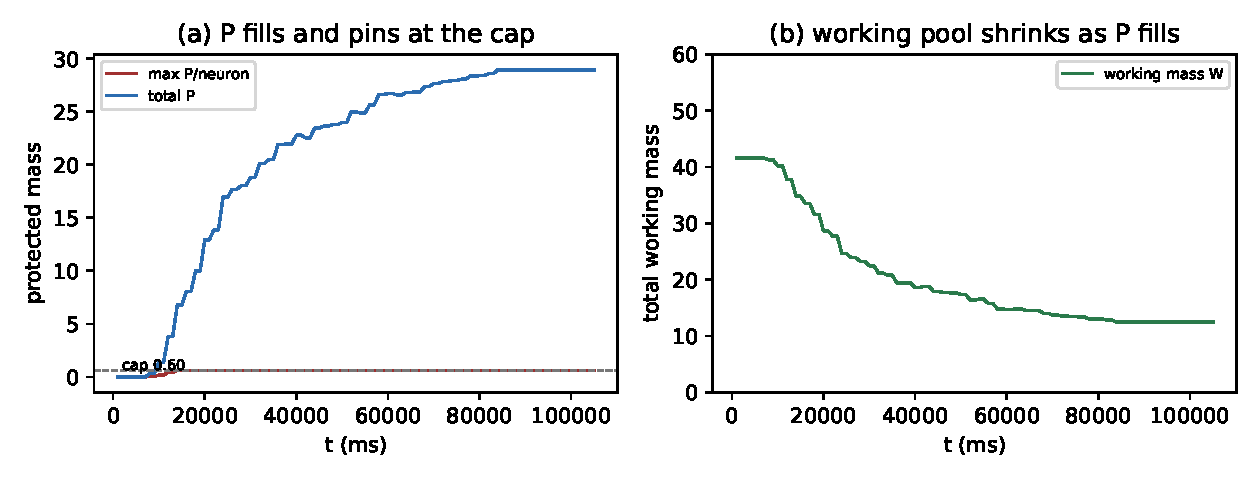
\includegraphics[width=\linewidth]{figures/fig6-protection.pdf}
\caption{\textbf{CLLA bounded protection: stability at the cap.}
Per-snapshot (1 s) trajectories of the previously-aborting
s424242-il cell under the bounded amendment: per-neuron protected mass
\(P\) rises to and pins at the 0.60 cap; total protected mass grows as
more neurons fill; the working pool \(W\) shrinks to the residual
budget as protection fills; zero failures (all 12 runs complete)
\cite{bbounded}.}
\label{fig:protection}
\end{figure}